\documentclass{article}
\usepackage[UTF8]{ctex}
\usepackage[a4paper,top=2cm,bottom=2cm,left=3cm,right=3cm]{geometry}
\usepackage{amsmath,amssymb}
\DeclareMathOperator*{\argmax}{arg\,max}
\DeclareMathOperator*{\argmin}{arg\,min}
\DeclareMathOperator{\softmax}{softmax}
\DeclareMathOperator{\rank}{rank}
\DeclareMathOperator{\concat}{concat}
\usepackage{booktabs}
\usepackage{array}
\usepackage{graphicx}
\usepackage{float}
\usepackage{adjustbox}
\usepackage{longtable}
\usepackage{pdflscape}
\usepackage{afterpage}
\AtBeginDvi{\special{pdf:minorversion 7}}
\usepackage[authoryear,round]{natbib}
\usepackage{hyperref}
\hypersetup{colorlinks=true,linkcolor=blue,citecolor=blue,urlcolor=blue}
\setlength{\emergencystretch}{3em}

% 让较大的浮动体与正文共享同一页，而不是被推到纯浮动页上居中、上下都留白。
\setcounter{topnumber}{3}
\setcounter{bottomnumber}{2}
\setcounter{totalnumber}{4}
\renewcommand{\topfraction}{0.9}
\renewcommand{\bottomfraction}{0.9}
\renewcommand{\textfraction}{0.05}
\renewcommand{\floatpagefraction}{0.85}
\renewcommand{\thetable}{\Roman{table}}
\title{资源约束下面向双语铁路职业教育的知识增强型大语言模型领域适配}
\author{}
\date{}

\begin{document}
\maketitle

\begin{abstract}

\textbf{目的：} 中国高铁技术的国际化应用不断扩大，对双语职业教育的需求持续增长，但铁路规章、专业术语和教学材料在中文与英文之间仍难以稳定获取。由于多数职业院校和地方研究团队的计算资源有限，本研究构建并评估一种可在单台工作站上完成适配与评估的铁路领域大语言模型，用于回答双语铁路问题。

\textbf{方法：} 本研究用两种方法应对该问题。第一种是混合证据融合方法：以倒数排名融合（RRF）融合 BM25 词法检索与 BGE-M3 稠密检索，并将排名最靠前的铁路证据段落作为知识上下文插入提示词用于作答。第二种是垂直领域适配方法：以 completion-only QLoRA 在经审核的铁路问答对上对 Qwen2.5-7B-Instruct 与 GLM-4-9B-Chat-HF 进行领域特化，基座权重以 4-bit NF4 冻结。两种方法在同一单卡边界下，针对留出双语铁路数据集、对照原始模型与未适配的 Qwen3-14B 参考模型进行评估。

\textbf{结果：} 证据融合在两种语言上都取得了最高的检索质量，中文与英文的证据 Recall@5 分别达到 0.715 与 0.708，且融合中英双语字段取得了最佳的跨语言均衡。垂直微调将 Qwen2.5-7B 的留出字符级 F1 从中文 0.189 提升至 0.398，从英文 0.437 提升至 0.648。两种方法结合取得最佳答案质量：在融合证据条件下，Qwen QLoRA 的答案 F1 达到中文 0.660、英文 0.651；加入该证据后，所有被评估生成器在两种语言上的答案 F1 均有提升。

\textbf{原创性/价值：} 研究表明，词法—稠密证据融合与参数高效垂直适配是构建领域模型时互补而非可相互替代的两种机制，在专业垂直领域中尤其如此。在统一资源边界和统一留出协议下报告两种方法，可以区分来自检索到的铁路知识的增益与来自领域微调的增益，并为在无多卡训练条件下开发垂直领域语言模型提供了可复现的流程。

\textbf{关键词：} 铁路领域大语言模型；双语职业教育；混合检索；倒数排名融合；检索增强生成；QLoRA

\end{abstract}

\section{引言}

高铁建设、运营与技术合作的国际化扩大了双语职业教育的需求 \citep{lawrence2019hsr,xu2018education}。跨国家、跨语言环境工作的铁路从业人员与学习者，必须理解通常首先以中文编写的运营规章、安全规程、设备术语和教学材料。因此，实际困难并不只是翻译孤立的术语。教学支持必须把以任一语言提出的问题连接到正确的铁路知识，并产出始终停留在该知识边界内的答案。

通用大语言模型可以流畅地组织这类知识，但它们并未在特定铁路语料的术语、证据边界和程序性约定上接受过训练。面向铁路的研究已经构建了用于安全、轨道管理、故障预测与健康管理、司机辅助和交互式培训的专用模型 \citep{zheng2023trafficsafety,li2024rschat,song2025railway,wang2024phm,luo2025driver,li2025training,huang2026emergency}，而更宏观的综述仍将可靠性与部署列为交通领域的未解问题 \citep{wandelt2024transport}。这一文献中反复出现两个弱点。第一，这些模型通常针对单一任务和单一语言开发，因此不清楚同一思路能否迁移到双语职业教育场景——在该场景中，同一条知识需要在中文和英文下都被正确回答。第二，检索到的外部知识所带来的贡献，很少与模型适配所带来的贡献被分开度量，这使得人们难以判断观测到的改进究竟由哪一种机制产生。

计算资源的可获得性是第二个同样具有约束力的条件。许多职业院校和地方研究团队既无法维持多卡训练集群，也无法持续依赖商业云推理。因此，对参数规模较大的模型做全参数适配，恰恰在最需要铁路领域助手的机构中难以复现、难以长期维持。量化低秩适配提供了一条现实的替代路径：7B 或 9B 模型可以在单张 24 GB GPU 上完成领域特化，而基座权重保持冻结。资源约束因此是研究问题的一部分，而不是次要的部署细节。

本研究用两种方法应对该问题。

第一种方法针对知识获取，下文称为\emph{证据融合}。BM25 词法排序与 BGE-M3 稠密排序并行计算，并以倒数排名融合合并；排名最高的铁路证据段落会在生成之前插入提示词。正是这一方法使以任一语言提出的问题能够抵达正确的已审核铁路记录，并依据该记录而非参数化记忆来作答。

第二种方法针对领域行为，下文称为\emph{垂直适配}。completion-only QLoRA 在经审核的铁路问答对上训练低秩适配器，而 4-bit 量化的基座模型保持冻结，从而使模型学习铁路答案的用词与结构，而不需要全参数训练。

随后对两种方法进行评估。检索以证据级指标计分；适配以留出铁路问题上的前后对照计分；组合系统则在相同的缓存证据下跨五个生成器计分；每一种实验的资源开销都在同一台工作站上测量。该设计回答了现有铁路领域文献尚未回答的问题：改进的知识获取与改进的领域行为究竟是相互替代还是相互补充，以及在固定硬件预算内各自付出何种代价。

本研究作出三项贡献：

\begin{itemize}
\item 将混合词法—稠密证据融合应用于双语铁路职业教育问答，并表明融合检索在两种语言上都取得最佳证据召回率，且双语字段的索引构成给出最佳的跨语言均衡。
\item 将 completion-only QLoRA 垂直适配应用于两个模型家族，并以配对显著性检验量化留出双语增益。
\item 构建了高质量的中英文平行铁路语料集，并在同一批留出记录上给出一次受控的联合评估，表明两种机制互补但部分重叠，且在同一基座模型上垂直适配贡献的增益份额更大。
\end{itemize}

\section{相关工作}

本节回顾本研究依托的三条工作线索，说明每条线索实际作出了什么贡献，并指出仍然存在的缺口。

\subsection{铁路与交通领域语言模型}

第一条工作线索把通用语言模型适配到铁路与交通任务上。Zheng 等（2023）构建了交通安全指令语料，并把预训练模型微调为领域专家，表明领域指令微调改变的是任务行为而不仅是表层风格。Li 等（2024）构建了 RSChat——一个面向铁路安全知识的智能问答模型，这是与本研究的铁路职业教育问答系统最为接近的已发表先例。Song 等（2025）将语言模型特化到铁路轨道管理，并报告了在轨道管理问题上相对通用模型的领域增益。Luo 等（2025）开发了高速铁路司机辅助系统，其中语言模型在时刻表与信号约束下生成操作建议。Li 等（2025）评测了面向铁路系统的智能人机交互培训助手，其场景涵盖调度与职业培训，是该组中唯一明确涉及铁路教育的研究。

另有两项工作延伸了同一思路。Huang 等（2026）用检索增强模型生成城市轨道交通列车车门系统的应急处置方案，表明当所需流程无法被可靠记忆时，外部证据是必需的。Wang 和 Li（2024）综述了语言模型在铁路故障预测与健康管理中的应用潜力、局限与所需解决方案，Lahnalampi（2024）考察了其在铁路设计项目中的使用。在更宏观的层面，Wandelt 等（2024）综述了面向智能交通的语言模型，并得出结论：可靠性、领域接地与部署成本仍属未解问题。

这条线索确立的是：铁路任务能够从领域特定的语言建模中获益，且当答案取决于具体规章或流程时，检索成为必需。它没有确立的是双语场景：所综述的系统均在单一语言下构建与评估，因此跨语言检索问题——即同一份证据能否同等地服务于中文问题和英文问题——仍处于开放状态。

\subsection{检索增强生成与混合证据融合}

第二条工作线索提供了知识获取机制。Lewis 等（2020）提出检索增强生成，其中参数化生成器以从外部非参数化索引中检索到的文档为条件。这种组织方式与铁路职业教育直接相关，因为规章、术语记录和教学材料会随时间修订，而外部索引可以在不重新训练生成器的情况下更新。

在这一框架内，检索组件沿两个互补方向得到发展。Robertson 和 Zaragoza（2009）形式化了概率相关性框架及其 BM25 实例，当查询与文档共享设备名称、规章编号、标准代码等精确词项时，该方法依然表现强劲。Chen 等（2024）提出了 BGE-M3——一种多语言嵌入模型，可为语义相关但词面不同的文本生成稠密表示，这在中文问题与英文问题以不同措辞表达同一需求时尤为重要。由于两种检索器在不可通约的量纲上计分，Cormack 等（2009）提出了倒数排名融合，它仅使用排名位置合并有序列表，因而无需分数归一化。Hübscher 等（2021）研究了在动态且以沟通为中心的环境中，知识与流程描述应如何表示与呈现，这与一条领域记录应如何组织才能同时被人工审核者和下游模型使用相关。在法律文档场景中，Yang 等（2024）综述了长专业文档上的问答，表明检索策略与答案核验是该体裁中两个决定性的设计选择。Chang 等（2024）综述了大语言模型评估，主张不同能力需要不同指标，而不是单一的聚合分数。

这条线索因此提供了本研究的第一种方法：在排名层面融合的词法与稠密检索。然而，其评估以单语为主，且大多假设单语索引。当每一条知识都以两种语言存在时索引应如何组织，以及双语字段构成的索引是否优于特定语言索引，这些问题在该文献中尚无定论。

\subsection{参数高效垂直领域适配}

第三条工作线索提供了适配机制。Dettmers 等（2023）提出 QLoRA，其通过冻结的 4-bit NF4 量化基座模型反向传播到低秩适配器，把训练显存降低到足以在单台设备上微调数十亿参数模型的程度。Ding 等（2023）与 Wang 等（2025）综述了参数高效微调，梳理了适配器容量、可训练参数量与任务表现之间的权衡。Lv 等（2024）考察了有限资源下的全参数微调，记录了此类训练对量化、序列长度和优化器状态的敏感性——这正是本研究显式固定这些设置而非采用默认值的原因。

该文献中贯穿着一贯的警示：适配并不自动带来收益。Tian 等（2024）表明微调可以提升事实性，但 Barnett 等（2024）证明当评估协议不受控时，微调常常不如更简单的替代方案。在驱动本研究的教学场景中，Kasneci 等（2023）与 UNESCO（2023）指出事实可靠性、学习者过度依赖以及来源不透明是生成式模型进入教学的主要风险。Schwartz 等（2020）更一般地主张，预测质量应当与其计算成本一并报告，只报告质量会歪曲一种高效方法的价值。因此，仅凭适配器大小并不能确立低推理成本；在宣称适配增益之前，需要前后对照设计以及实测资源开销。

\subsection{研究缺口}

上述三条线索分别提供了领域动机、知识获取机制与适配机制，但尚未在同一个受控协议下被结合起来。铁路领域研究基本是单语的，且通常只报告单一机制。混合检索研究的索引设计基本是单语的，且很少测量资源开销。参数高效适配研究则很少检验当外部证据同样被提供时，所观测到的增益是否依然成立。

本研究通过把两种方法应用到同一个双语铁路语料、并在同一硬件边界下于同一批留出记录上评估，来填补这一缺口。由此可以一并回答三个问题：融合式双语检索是否比任一单一检索器改善证据获取；completion-only QLoRA 是否改善留出铁路问答；以及当适配后的模型同样接收融合证据时，两种增益是叠加的还是重叠的。

\section{方法}

\subsection{问题定义与资源边界}

任务是在经审核的规章、术语记录和职业教学材料上进行双语铁路问答。设 $\mathcal{D}$ 为受治理的铁路记录知识库，$q$ 为以中文或英文书写的提问。系统必须返回与提问语言一致的答案 $\hat{y}$：

\begin{equation}
\hat{y}=f_{\theta_0,\theta_A}\big(q,\;\mathcal{R}(q,\mathcal{D})\big),
\end{equation}

其中 $\mathcal{R}(q,\mathcal{D})$ 是检索函数返回的证据，$f$ 是基座权重 $\theta_0$ 冻结、由适配器权重 $\theta_A$ 承载领域适配的生成器。式（1）直接陈述了本研究的两条方法：$\mathcal{R}$ 是证据融合方法，$\theta_A$ 是垂直适配方法。当 $\mathcal{R}(q,\mathcal{D})=\varnothing$ 时，生成器仅凭参数化记忆作答，即贯穿全文的无检索基线条件。

资源边界为一台 NVIDIA RTX 3090 GPU，24 GB 显存与 32 GB 系统内存，不使用多卡训练，也不要求云端推理。记 $M$ 为某条件的峰值显存，则每一种配置都必须满足

\begin{equation}
M \le 24\ \text{GB},
\end{equation}

正因为式（2）对全部条件成立，所报告的分数才具有可比性。这一约束使 NF4 量化与低秩适配成为必需而非可选项，因为对所选 7B 与 9B 模型做全参数训练会超出该边界。

\subsection{总体框架}

\begin{figure}[!htbp]
\centering
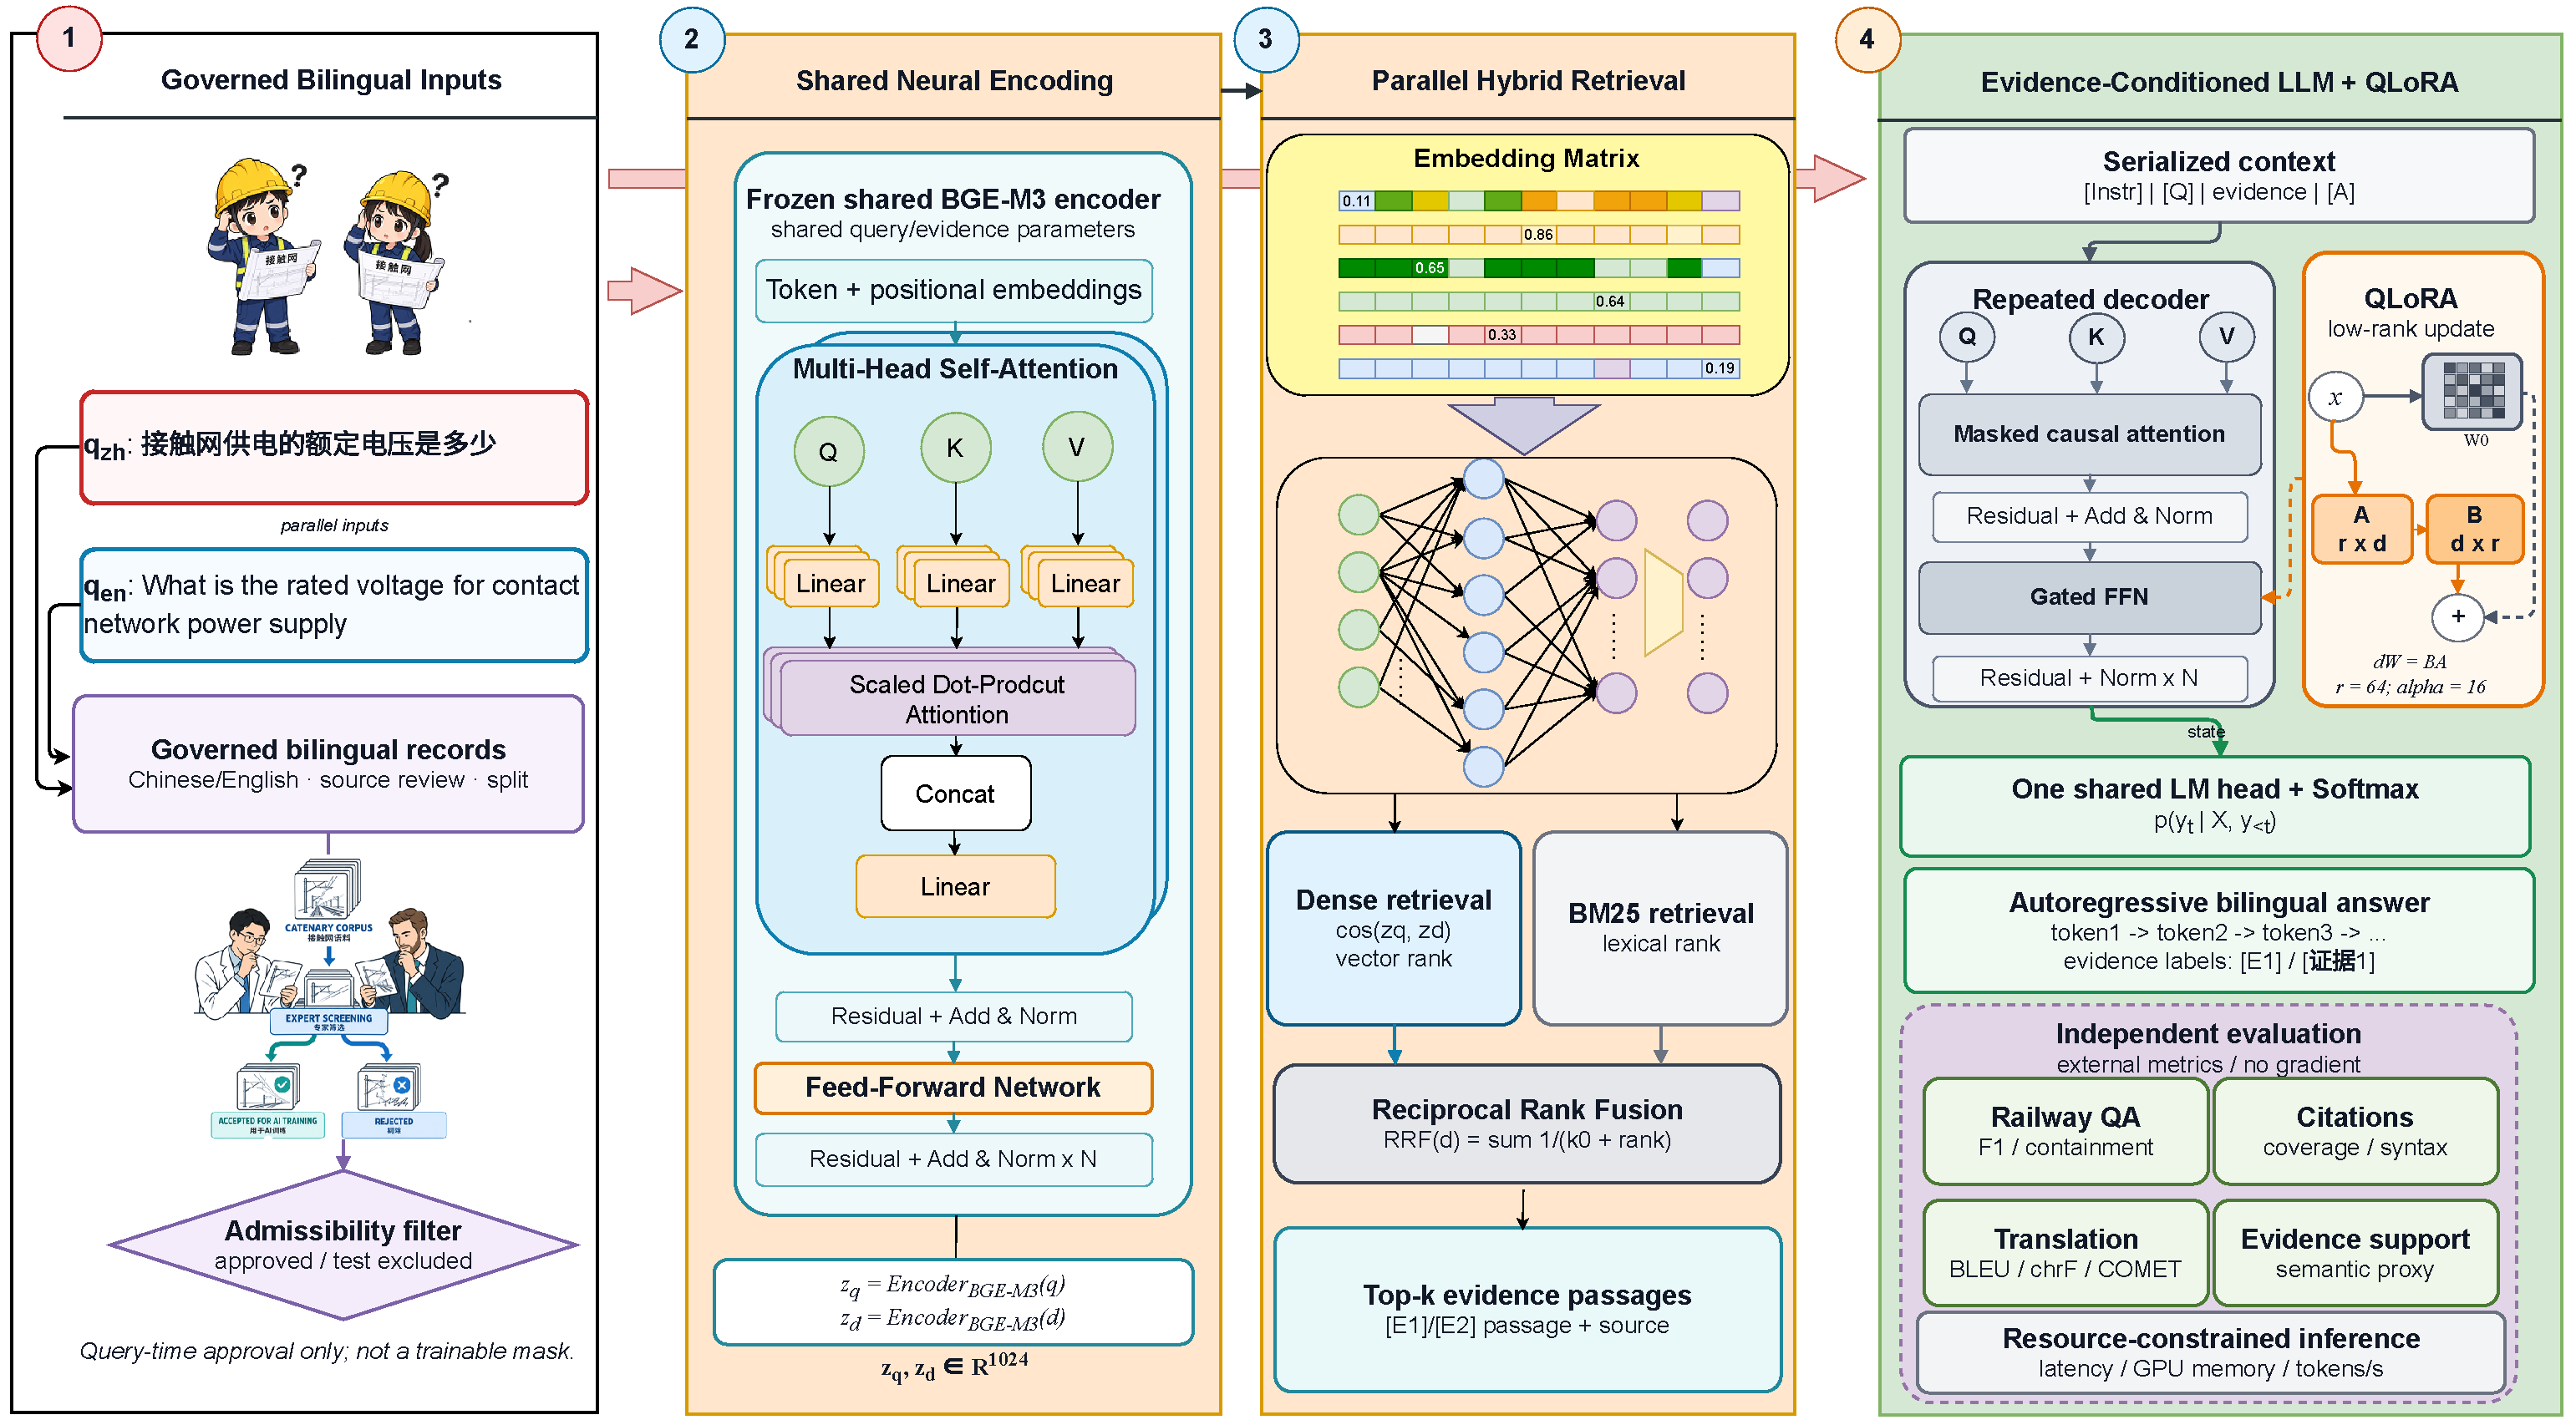
\includegraphics[width=0.92\linewidth,height=0.78\textheight,keepaspectratio]{figures/figure_01_neural_retrieval.pdf}
\caption{面向双语铁路问答的两种方法。（1）受治理的双语输入：中文查询 $q_{zh}$ 与英文查询 $q_{en}$ 指向同一条知识，准入过滤器仅保留已批准的配对。（2）共享神经编码：一个冻结的 BGE-M3 编码器把查询与候选证据映射到同一个 1024 维空间。（3）带证据融合的并行混合检索：稠密检索器计算余弦相似度，BM25 计算词法重叠度，倒数排名融合把两个排序合并为一个 top-$k$ 证据集合。（4）证据条件化生成与垂直适配：序列化上下文 $[\text{Instr}]\,|\,[\text{Q}]\,|\,\text{evidence}\,|\,[\text{A}]$ 由重复的因果解码器解码，其冻结权重 $W_0$ 接受低秩更新 $dW=BA$（秩 64，alpha 16）。上方路径为证据融合，下方路径为垂直适配；两者汇合于同一个生成器，从而可以区分各自的贡献。}
\label{fig:neural-retrieval-qlora}
\end{figure}

图 1 把两种方法放在同一个系统上。证据融合改变生成器被允许看到的内容，而垂直适配改变生成器作答的方式。由于两种机制作用于架构中的不同位置，可以通过固定其中之一、变动另一个来区分各自的贡献。

\subsection{方法一：带证据融合的双语混合检索}

第一种方法解决知识获取问题。铁路问题混杂着精确标识符与改述后的技术描述，单一检索器无法同时应对两者。因此该方法并行计算两个排序，并在排名层面加以合并。

词法排序用 BM25 对候选段落 $d$ 与查询 $q$ 计分 \citep{robertson2009bm25}：

\begin{equation}
\operatorname{BM25}(q,d)=\sum_{t\in q}\operatorname{IDF}(t)\cdot
\frac{f(t,d)\,(k_1+1)}{f(t,d)+k_1\left(1-b+b\,\frac{|d|}{\mathrm{avgdl}}\right)}
\cdot\bigl(1+0.05\min\!\left(f(t,q),3\right)\bigr),
\end{equation}

其中 $f(t,d)$ 是词项 $t$ 在 $d$ 中的频次，$f(t,q)$ 是其在查询中的频次，$|d|$ 是段落长度，$\mathrm{avgdl}$ 是索引中的平均段落长度，$k_1$ 与 $b$ 分别控制词频饱和与长度归一化。实现中取 $k_1=1.5$、$b=0.75$，末尾因子对出现多于一次的查询词项给予轻微加权，并在出现三次时饱和。本语料规模足够小，索引常驻内存，因此不涉及外部检索库。并且

\begin{equation}
\operatorname{IDF}(t)=\ln\!\left(\frac{N-n(t)+0.5}{n(t)+0.5}+1\right)
\end{equation}

其中 $N$ 是索引段落总数，$n(t)$ 是包含 $t$ 的段落数。式（3）奖励精确重叠，正是这一点保住了稠密编码器可能模糊掉的设备名称、条款编号与标准代码。

稠密排序用 BGE-M3 对查询与段落编码 \citep{chen2024bgem3}，并以余弦相似度计分：

\begin{equation}
s_{\mathrm{dense}}(q,d)=\frac{\mathbf{e}_q^{\top}\mathbf{e}_d}{\lVert\mathbf{e}_q\rVert_2\,\lVert\mathbf{e}_d\rVert_2},
\end{equation}

其中 $\mathbf{e}_q,\mathbf{e}_d\in\mathbb{R}^{1024}$。式（5）奖励语义等价，正是这一点使一个与英文段落没有表层词项重合的中文查询仍能召回该段落。

由于式（3）与式（5）不在同一量纲上，两个排序以倒数排名融合合并 \citep{cormack2009rrf}：

\begin{equation}
\operatorname{RRF}(d)=\sum_{r\in\{\mathrm{BM25},\,\mathrm{dense}\}}\frac{1}{k_0+\rank_r(d)},
\end{equation}

其中 $\rank_r(d)$ 是 $d$ 在排序 $r$ 中的位置，$k_0$ 是平滑常数。未出现在某检索器候选列表中的段落，对该检索器的贡献为零。式（6）只依赖排名位置，因此不需要在词法检索器与稠密检索器之间做分数校准。每个检索器的候选池固定为 50，取 $k_0=60$，且融合在最终截断点选定之前完成。

融合后的列表被截断为前 $k$ 个段落，并以知识上下文的形式序列化进提示词：

\begin{equation}
\mathcal{R}(q,\mathcal{D})=\underset{d\in\mathcal{D}_{\mathrm{adm}}}{\operatorname{top}\text{-}k}\ \operatorname{RRF}(d),
\end{equation}

其中 $\mathcal{D}_{\mathrm{adm}}$ 是知识库中的准入子集，提示词则拼接为

\begin{equation}
x=\big[\,\text{Instr}\,\big]\;\big|\;\big[\,q\,\big]\;\big|\;\big[E_1\big]\ldots\big[E_k\big]\;\big|\;\big[\,\text{A}\,\big],
\end{equation}

其中每个 $E_i$ 在提示词中被渲染为带编号的标签、其来源文档与段落文本，而检索对象同时携带评估所需的记录标识符、来源文档与任务类型。式（8）是第一种方法把控制权交给生成器的节点：标签 $[E_i]$ 为模型提供了一个可寻址的证据集合，而实验把 $k$ 从一变动到八，以度量提供多少证据是值得的。

本实现有两点设计选择值得说明。第一，查询与证据使用同一个编码器，因此查询时无需跨语言对齐步骤。第二，留出记录在排名之前即被移除：词法索引在构建时就排除了测试划分与预留 RAG 测试记录，稠密查询也在其数据库谓词中携带同样的排除条件。这保证了留出记录不可能作为其自身问题的证据被返回。仅批准记录是一个独立的控制项，它在返回候选时执行，而不是被假定为语料的既有属性；两种控制项在结果中分别报告。

\subsection{方法二：completion-only QLoRA 垂直适配}

第二种方法解决领域行为问题。通用模型会生成流畅但语域不当的答案，遗漏铁路答案中应有的程序性细节，或以改述而非条款内容来回答规章问题。该方法通过在经审核的铁路问答对上训练低秩适配器、同时保持基座模型冻结，来纠正这一点。

对于预训练权重矩阵 $W_0\in\mathbb{R}^{d\times k}$，适配后的前向传播为

\begin{equation}
h=W_0x+\Delta Wx=W_0x+\frac{\alpha}{r}BAx,
\end{equation}

其中 $A\in\mathbb{R}^{r\times k}$ 与 $B\in\mathbb{R}^{d\times r}$ 是可训练的低秩因子，$r$ 是秩，$\alpha$ 是固定的缩放常数 \citep{dettmers2023qlora}。只有 $A$ 与 $B$ 接收梯度，因此可训练参数量为 $r(d+k)$ 而非 $dk$；取 $r=64$ 时这只是完整矩阵的一小部分，也正是该方法能够满足式（2）的原因。

冻结的基座权重以 4-bit NF4 格式存储。一个权重块在前向传播前以逐块的缩放与零点常数反量化：

\begin{equation}
W_0 \approx s_b\left(q_b-c_b\right),
\end{equation}

其中 $q_b$ 是量化后的块，$s_b$ 与 $c_b$ 是该块的缩放与偏移。式（10）是基座权重的一种有损表示，而式（9）中的适配器正是在该降低的精度下恢复任务能力。

监督只施加在答案词元上。记答案词元处 $m_t=1$、提示词词元处 $m_t=0$，训练目标为

\begin{equation}
\mathcal{L}(\theta_A)=-\frac{1}{\sum_t m_t}\sum_t m_t\log p_{\theta_0,\theta_A}\!\left(y_t\mid y_{<t},x\right),
\end{equation}

其中 $\theta_0$ 表示冻结的 NF4 基座权重，$\theta_A=\{\theta_A^{(l)}\}_{l=1}^{L}$ 表示各层中可训练的适配器。式（11）正是该方法被称为 completion-only 的原因：掩蔽提示词位置使模型不至于把容量花在复现指令上，而是集中到铁路答案上，同时使训练信号与式（1）所定义的推理期任务保持一致。

适配语料仅由已批准记录构建，并按知识对标识符、任务类型与来源文档划分。同一条知识的中英文变体总是被分到同一划分，因此一个双语对不可能横跨训练与留出边界，且没有任何知识对标识符在划分之间共享。completion-only 掩蔽把每个提示词词元标注为 $-100$；损失仅在答案词元上计算。

\subsection{评估协议}

评估模块位于生成器之外且不携带梯度，因此本研究报告的每一项量值都是外部测量，而不是训练信号。它涵盖作为主要结果的铁路问答分数，同时也涵盖系统部署后所支持的后续延伸用途：依据证据对生成的答案进行引用、在中文与英文之间翻译答案、检查其论断是否被检索到的段落所支持，以及在资源受限推理边界下测量时延与显存。本小节其余部分定义主要结果所依据的指标。

检索在证据层面而非记录层面计分，因为另一条准入记录可能合法地包含回答该问题所需的证据。当且仅当前 $k$ 个候选中至少有一个满足匹配规则时，证据等价 Recall@$k$ 取值为一：

\begin{equation}
\operatorname{Recall@}k=\frac{1}{|\mathcal{Q}|}\sum_{q\in\mathcal{Q}}
\mathbf{1}\!\left[\exists\, d\in \operatorname{top}\text{-}k(q):\ \operatorname{match}(d,q)\right],
\end{equation}

其中 $\operatorname{match}(d,q)$ 在以下情形成立：候选与金标证据共享记录标识符；空白归一化后的金标证据与候选证据在任一方向上相互包含；或候选来自同一来源文档且包含金标答案。平均倒数排名在首个匹配候选的排位上计算：

\begin{equation}
\operatorname{MRR}=\frac{1}{|\mathcal{Q}|}\sum_{q\in\mathcal{Q}}\frac{1}{\rank_q^{*}},
\end{equation}

其中 $\rank_q^{*}$ 是查询 $q$ 的首个匹配候选项的排位，若没有候选匹配则贡献为零。

生成以预测 $\hat{y}$ 与参考答案 $y$ 之间的字符级重叠计分，在答案归一化并去除空白之后，于字符的多重集上计算：

\begin{equation}
P=\frac{|\hat{y}\cap y|}{|\hat{y}|},\qquad
R=\frac{|\hat{y}\cap y|}{|y|},\qquad
F1=\frac{2PR}{P+R}.
\end{equation}

在检索增强实验中，同一重叠改为在中文字符以及小写化后的拉丁字母与字母数字词元上计算。两种定义各自在其所属设置内报告，不被视为可互换的绝对分数。参考包含率与 $F1$ 一并报告，作为归一化参考答案是否出现在预测中的更严格指标。

所有生成器比较均使用配对样本。条件之间的差异以双侧配对 Wilcoxon 检验、配对效应量

\begin{equation}
d_z=\frac{\bar{d}}{s_d},
\end{equation}

其中 $\bar{d}$ 是逐样本差值的均值、$s_d$ 是其标准差，并在预先设定的比较族上作 Holm 校正。均值指标附带 2{,}000 次重抽样的 bootstrap 95\% 置信区间。

资源开销在 30 条中文短问题、30 条英文短问题和 30 条面向规章的长上下文问题上测量，每个条件在开始时包含一条预热提示词与三次实测重复，合计每个条件 270 次测量。报告的量为峰值与静态预留显存、首词元时延、平均端到端时延与生成吞吐。

\subsection{实验配置}

表 I 定义了单工作站边界与共享设置。所有检索、适配与生成条件均在该边界内执行，未使用多卡训练或云端推理。

\begin{table}[ht]
\centering
\caption{单工作站实现与实验配置。}

\begin{tabular}{p{0.28\linewidth}p{0.64\linewidth}}
\toprule
组件 & 正式设置 \\
\midrule
数据库 & PostgreSQL 16.14；pgvector 0.8.4 \\
嵌入模型 & BAAI/bge-m3；1{,}024 维；冻结的共享编码器 \\
适配生成器 & Qwen2.5-7B-Instruct；GLM-4-9B-Chat-HF \\
参考生成器 & 通过 Ollama 0.19.0 调用的 Qwen3-14B（未适配） \\
检索 & BM25 与稠密检索，各取 50 个候选；RRF 取 $k_0=60$ \\
训练 & NF4 QLoRA；秩 64；alpha 16；dropout 0.05；一个 epoch；随机种子 42 \\
优化 & 学习率 2e-4；批大小 1；16 步梯度累积；预热比例 0.03 \\
序列长度 & 最大 1{,}024 词元 \\
解码 & 贪心；温度 0；top-$p$ 为 1 \\
硬件边界 & 单张 RTX 3090 24 GB；32 GB 内存；不使用多卡或强制云端推理 \\
统计分析 & 2{,}000 次 bootstrap 重抽样；配对 Wilcoxon；Cohen's \emph{d}\textsubscript{z}；Holm 校正 \\
软件 & Linux；Python 3.11.15；PyTorch 2.11.0；Transformers 5.12.1；PEFT 0.18.1；bitsandbytes 0.49.2；Ollama 0.19.0 \\
\bottomrule
\end{tabular}
\end{table}

两个被适配模型需要不同的适配器挂载位置，因为其注意力与前馈模块的命名并不一致。Qwen2.5-7B 暴露相互独立的 gate 与 up 投影，而 GLM-4-9B 使用融合的 gate-up 投影，因此目标模块列表是模型特定的。表 II 记录了由此得到的适配矩阵与可训练参数量。

\begin{table}[ht]
\centering
\caption{垂直适配配置与可训练参数量。}

\small
\begin{adjustbox}{max width=\linewidth}
\begin{tabular}{llllrl}
\toprule
模型 & 检查点 & 量化 & 目标模块 & 可训练参数 & 占比 \\
\midrule
Qwen2.5-7B & Qwen/Qwen2.5-7B-Instruct & NF4 4-bit & q, k, v, o, up, down, gate & 161{,}480{,}704 & 3.58\% \\
GLM-4-9B & THUDM/glm-4-9b-chat-hf & NF4 4-bit & q, k, v, o, down, gate\_up & 190{,}382{,}080 & 3.45\% \\
\bottomrule
\end{tabular}
\end{adjustbox}
\end{table}

“占比”一列报告的是可训练参数占量化训练过程可见参数的比例，而不是占原始全精度模型的比例。基座模型架构及其后训练脉络见相应技术报告 \citep{qwen2024technical,glm2024chatglm}，未适配的参考模型见 \citep{qwen2025technical}。

\section{结果}

\subsection{语料与实验样本}

受治理的知识库包含 37{,}661 条已批准记录与 37{,}109 条完整双语记录，其中中文字段与英文字段共享同一个知识对标识符。来源包括铁路术语、运营与安全规章，以及职业教材或概念材料。从已批准的双语对中，按任务上限选出 7{,}614 对，并按知识对标识符以 80/10/10 划分为 12{,}178 条训练、1{,}524 条验证与 1{,}526 条留出记录，两种语言各半。三个划分之间的知识对重叠均为零。留出划分包含 4 个来源文档下的 763 个知识对；由于四分之三的术语对触及了单任务上限，冻结样本按该比例以术语、规章和教材任务为主。

从留出划分中抽取两个评估样本。独立双语问答样本在两种语言下使用全部 763 对。跨来源检索增强样本使用 400 对与 800 条语言特定查询，覆盖 17 种任务类型下的 150 个规章对、127 个术语对与 123 个教材或概念对。所有生成器使用同样的 400 对与同样的缓存证据，因此生成器之间的差异不可能来自检索上下文的差异。

\subsection{证据融合在两种语言上都提升检索}

表 III 报告了在 400 对跨来源样本上的检索比较。由此可得到三点观察。

\begin{table}[ht]
\centering
\caption{400 个留出知识对上的检索质量与时延。}

\small
\begin{adjustbox}{max width=\linewidth}
\begin{tabular}{>{\raggedright\arraybackslash}p{0.19\linewidth}lrrrrr}
\toprule
检索 & 语言 & 证据 R@1 & 证据 R@3 & 证据 R@5 & MRR & 平均时延（ms） \\
\midrule
BM25 & 中文 & 0.520 & 0.595 & 0.620 & 0.560 & \textbf{69.5} \\
稠密 & 中文 & 0.518 & 0.653 & 0.690 & 0.588 & 134.4 \\
融合 & 中文 & \textbf{0.570} & \textbf{0.675} & \textbf{0.715} & \textbf{0.628} & 217.6 \\
BM25 & 英文 & \textbf{0.570} & \textbf{0.670} & 0.685 & 0.620 & \textbf{59.0} \\
稠密 & 英文 & 0.463 & 0.553 & 0.580 & 0.509 & 134.4 \\
融合 & 英文 & \textbf{0.570} & 0.668 & \textbf{0.708} & \textbf{0.620} & 209.2 \\
\bottomrule
\end{tabular}
\end{adjustbox}
\end{table}

第一，两种检索器不可互换，且其弱点依赖于语言。BM25 是英文上最强的单一检索器，证据 Recall@1 达 0.570、MRR 达 0.620，这反映了大量英文查询与其证据共享精确术语。稠密检索则是在召回层级高于一时更强的中文单一检索器，证据 Recall@5 达 0.690，而 BM25 为 0.620，这反映了中文查询更多是改述而非词项匹配。两者均不占优，这正是融合能够起作用的前提。

第二，融合同时优于两者。融合后的排序在中文（0.715）与英文（0.708）上都取得最高的证据 Recall@5，并在两种语言上取得最高的 MRR（0.628 与 0.620）。增益在两种检索器分歧最大处最为明显：在中文上，融合把 Recall@1 从 0.520 提升到 0.570，而单独使用稠密检索时为 0.518，说明词法排序仍然贡献了稠密排序遗漏的候选。

第三，该改进并非没有代价。平均检索时延从 BM25 的 69.5 ms 与稠密检索的 134.4 ms 上升到中文融合条件的 217.6 ms，因此融合是质量与时延之间的权衡，而不是一致的效率优势。在本冻结实验中，过滤到已批准记录不改变任何结果，因为受治理语料在 37{,}664 条记录中含有 37{,}661 条已批准记录，因此准入索引与已批准索引在实践中是同一个索引；该过滤器关乎协议的正确性，而非实测分数。

\begin{figure}[!htb]
\centering
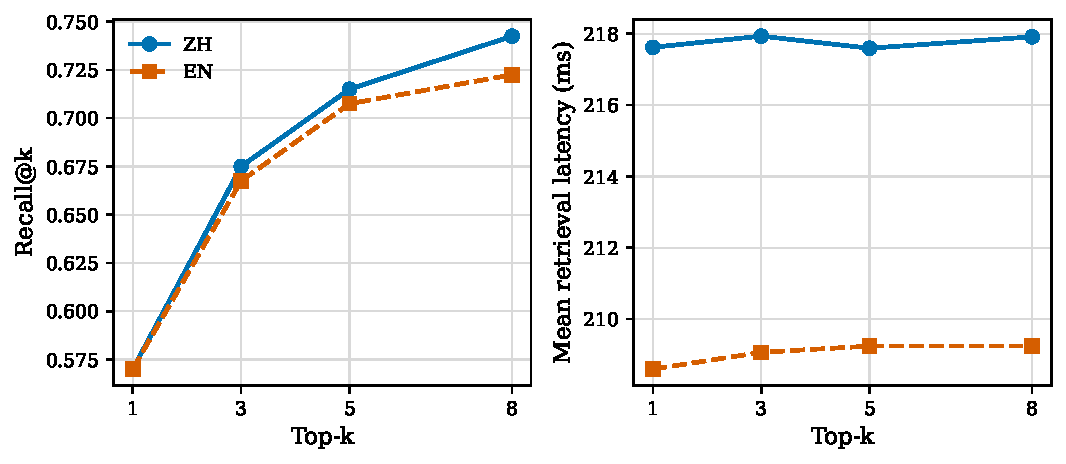
\includegraphics[width=0.72\linewidth,keepaspectratio]{figures/figure_03_top_k_quality_latency.pdf}
\caption{最终证据截断点对融合检索的影响。召回率从 top-1 的 0.570 上升到 top-8 时中文的 0.743 与英文的 0.723，而平均检索时延保持在约 218 ms 与 209 ms，因为上游候选池固定为每个检索器 50 个段落。因此，提高融合截断点可以在不显著改变检索时间的情况下改善证据覆盖。}
\end{figure}

图 2 展示了最终证据截断点如何与质量和时延相互作用。召回率随 $k$ 单调上升，从 $k=1$ 时的 0.570 上升到 $k=8$ 时中文的 0.743 与英文的 0.723；单步增幅最大的是 $k=1$ 到 $k=3$ 之间，此后曲线趋于平缓。在同一区间内检索时延几乎持平，中文保持在 218 ms 附近、英文保持在 209 ms 附近，因为每个设置都复用同样的 50 候选池，改变的只是截断点。因此，提供给生成器的证据量几乎可以在不增加检索成本的情况下提升，尽管更长的上下文仍会消耗生成时间与显存。

\subsection{双语索引构成}

由于每条知识都以两种语言存在，索引可以由中文字段、英文字段、来源证据字段，或同时由两种语言字段构建。四种构成在同一批样本上进行了比较，结果支持采用双语索引。

在融合检索下，双语索引取得最佳的跨语言均衡，中文证据 Recall@5 为 0.718、英文为 0.675，均值为 0.696。英文字段索引在英文上更好（0.713），但中文明显较弱（0.560）；中文字段索引在中文上更好（0.653），但英文较弱（0.530）。来源证据索引整体最弱（中文 0.638、英文 0.448）。因此，特定语言索引会在其自身语言上取胜而在另一种语言上失利，这对双语职业助手而言是错误的取舍——学习者可能用任一语言询问同一条知识。索引两种语言字段，正是使两种语言保持在同一可比区间内、而无需按语言切换索引的原因。

\subsection{垂直适配提升留出铁路问答}

表 IV 报告了在全部 763 对留出集上的前后对照，评估时不使用检索，从而使测量分离出第二种方法。

\begin{table}[ht]
\centering
\caption{垂直适配前后留出铁路问答表现（字符级 F1，每格 $n=763$）。}

\small
\begin{adjustbox}{max width=\linewidth}
\begin{tabular}{llcccc}
\toprule
模型 & 语言 & 原始 F1（95\% CI） & 适配后 F1（95\% CI） & 绝对增益 & Cohen's \emph{d}\textsubscript{z} \\
\midrule
Qwen2.5-7B & 中文 & 0.189（0.175--0.204） & \textbf{0.398}（0.376--0.422） & +0.209 & 0.569 \\
Qwen2.5-7B & 英文 & 0.437（0.419--0.455） & \textbf{0.648}（0.632--0.664） & +0.211 & 0.634 \\
GLM-4-9B & 中文 & 0.192（0.179--0.207） & 0.410（0.384--0.436） & +0.218 & 0.614 \\
GLM-4-9B & 英文 & 0.498（0.481--0.515） & 0.552（0.522--0.582） & +0.054 & 0.146 \\
\bottomrule
\end{tabular}
\end{adjustbox}
\end{table}

四个配对增益在 Holm 校正后均保持显著，各条件的校正后 $p$ 值均低于 0.01。两个模型家族的中文增益都很大，原始分数大约翻倍：Qwen2.5-7B 从 0.189 升至 0.398，GLM-4-9B 从 0.192 升至 0.410。英文表现则因模型而异。Qwen2.5-7B 显著提升，从 0.437 到 0.648；而 GLM-4-9B 仅从 0.498 提升到 0.552，配对效应量低至 0.146。因此，把两种语言合并会掩盖模型之间的真实差异，全文因此始终分别报告两种语言。

这一相对格局在另一方面也具有信息量。适配之前，GLM-4-9B 是更强的英文模型，两个模型在中文上相当。适配之后，Qwen2.5-7B 在两种语言上都是最强的模型，其双语差距在绝对量上从 0.248 变为 0.250，但英文的相对优势从 131\% 收窄到 63\%。因此，适配在最弱的环节帮助最大，这与该方法补齐缺失的领域词汇、而非统一抬升全部输出的解释一致。

图 3 展示了产生这些增益的优化行为。两个模型在单轮训练开始时都急剧降低训练损失，随后趋于平缓，且轮末验证测量值紧贴最终训练损失区间，表明在资源限制下的单轮计划已足以拟合适配集，两条曲线之间未见明显发散。Qwen 在训练曲线与验证曲线上都低于 GLM，这与其更强的留出结果一致。

\begin{figure}[!htb]
\centering
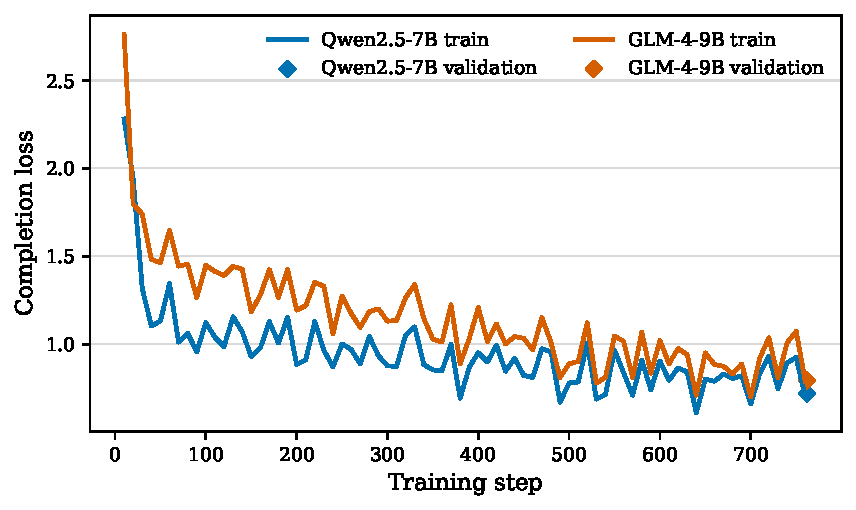
\includegraphics[width=0.72\linewidth,keepaspectratio]{figures/figure_04_training_validation_loss.pdf}
\caption{单轮 completion-only QLoRA 优化。两个模型的训练损失都迅速下降随后趋于平缓；菱形标记轮末验证测量值，二者都贴近最终训练区间。Qwen2.5-7B 在两条曲线上都低于 GLM-4-9B，与其更强的留出结果一致。曲线支持在资源限制内成功完成优化，但不构成更长训练计划或重复随机种子下的结论。}
\end{figure}

\subsection{证据融合与垂直适配的联合评估}

随后两种方法被联合使用。五个生成器在相同的 400 对样本、相同的缓存证据下，接受三种检索条件的评估：无检索、BM25 检索，以及融合的已批准检索。表 V 报告了无检索与融合证据之间的比较，并把适配后的模型与原始模型以及更大的未适配参考模型并列。

\begin{table}[ht]
\centering
\caption{无检索与融合证据条件下的答案质量（每格 $n=400$ 条查询）。}

\small
\begin{adjustbox}{max width=\linewidth}
\begin{tabular}{>{\raggedright\arraybackslash}p{0.17\linewidth}cccccc}
\toprule
生成器 & 无检索（中/英） & BM25（中/英） & 融合（中/英） & 融合增益（中/英） & Holm \emph{p}（中/英） \\
\midrule
Qwen2.5-7B 原始 & 0.262 / 0.306 & 0.406 / 0.433 & 0.402 / 0.440 & +0.141 / +0.133 & 1.9e-39 / 2.3e-42 \\
GLM-4-9B 原始 & 0.230 / 0.269 & 0.291 / 0.314 & 0.298 / 0.318 & +0.067 / +0.048 & 1.1e-22 / 9.6e-31 \\
Qwen2.5-7B QLoRA & 0.630 / 0.574 & \textbf{0.674} / 0.644 & 0.660 / \textbf{0.651} & +0.030 / +0.078 & 1.3e-06 / 1.4e-11 \\
GLM-4-9B QLoRA & 0.398 / 0.331 & 0.482 / 0.355 & 0.476 / 0.351 & +0.077 / +0.020 & 3.2e-09 / 9.4e-03 \\
Qwen3-14B 未适配 & 0.295 / 0.336 & 0.439 / 0.464 & 0.442 / 0.454 & +0.147 / +0.118 & 6.7e-32 / 7.6e-29 \\
\bottomrule
\end{tabular}
\end{adjustbox}
\end{table}

加入融合证据后，每一个生成器与每一种语言相对无检索的答案 F1 都有提升，且全部十项比较在 Holm 校正后仍然显著。然而增益幅度强烈依赖于生成器。原始 Qwen2.5-7B 中文增益 0.141、英文 0.133，未适配的 Qwen3-14B 增益 0.147 与 0.118，而适配后的 Qwen2.5-7B 仅增益 0.030 与 0.078。GLM-4-9B 呈现同样的格局，其增益在适配前为 0.067 与 0.048，适配后为 0.077 与 0.020。这正是两种部分重叠机制的预期特征：一旦适配后的模型已经在参数中带有铁路知识，检索证据的边际价值就变小，尽管该证据仍然带来显著增量。

对于实践问题而言，绝对排名才是关键。适配后的 Qwen2.5-7B 在每一种语言与检索条件下都是最强的生成器，在融合证据下达到中文 0.660、英文 0.651，在 BM25 下中文达到 0.674。它大幅超过未适配的 14B 参考模型：中文 0.660 对 0.442，英文 0.651 对 0.454，表明领域适配不可被规模替代。反向结论同样成立：原始 Qwen2.5-7B 在融合证据下达到 0.402 与 0.440，仍远低于其适配版本在无任何检索时的水平，因此检索知识也不可被适配替代。在固定硬件预算内，要取得最佳结果，两种方法缺一不可。

最后一项比较针对检索策略本身。BM25 与融合检索在答案质量上的排序并不一致：在中文上，BM25 对 Qwen2.5-7B QLoRA 更优（0.674 对 0.660），对未适配的 Qwen3-14B 在两种语言上都更优；而在英文上，融合检索对 Qwen2.5-7B QLoRA 更优（0.651 对 0.644），对原始 Qwen2.5-7B 在两种语言上都更优。融合索引具有更高的证据召回率，但这并不总能转化为更高的答案重叠，这意味着检索策略的最终选择应当在将要部署的那个生成器上验证，而不能只看检索指标。

\subsection{资源开销}

表 VI 报告了每个条件在 270 次测量上的实测开销。

\begin{table}[ht]
\centering
\caption{每个条件 270 次生成下的实测资源开销。}

\small
\begin{adjustbox}{max width=\linewidth}
\begin{tabular}{llrrrr}
\toprule
模型 & 条件 & 峰值预留显存（GiB） & 平均时延（s） & 吞吐（tokens/s） & 失败次数 \\
\midrule
Qwen2.5-7B & 原始 & 5.49 & 4.01 & 31.9 & 0 \\
Qwen2.5-7B & 适配后 & 16.11 & 6.83 & 17.5 & 0 \\
GLM-4-9B & 原始 & 6.76 & 5.65 & 22.7 & 0 \\
GLM-4-9B & 适配后 & 19.49 & 2.63 & 11.9 & 0 \\
Qwen3-14B（Ollama） & 未适配 & 14.26 & 1.63 & 78.5 & 0 \\
\bottomrule
\end{tabular}
\end{adjustbox}
\end{table}

五个条件全部完成，未出现执行失败或显存不足中断，因此式（2）对每一种配置都成立，包括预留显存为 19.49 GiB 的适配后 9B 模型。这正是核心的可行性结论：表 V 中质量最高的配置在目标工作站上仍然可执行。

在解读显存与时延两列时需要两点注意。预留显存包含缓存分配器的保留量，不应被读作活跃张量所占用的内存，因此原始与适配后显存数值之差会高估适配器本身的固有开销；可训练的适配器仅含 161.5M 与 190.4M 参数（表 II），相对于两行之间数 GiB 的差距只是很小的一部分。Qwen3-14B 一行经不同的运行时测量，报告的是 GPU 进程显存而非 PyTorch 预留显存，因此该行的跨后端比较仅为描述性的。GLM-4-9B 适配后 2.63 s 的时延并非效率优势：它反映的是异常短或为空的输出，而 11.9 tokens/s 的低吞吐与该解读一致，因此该条件被排除在任何效率结论之外。

图 4 把质量与开销放在同一组坐标轴上。适配后的 Qwen2.5-7B 在两个面板中都处于质量最高的位置，同时保持在 24 GB 边界之下，这正是本研究报告的质量—资源权衡。原始模型的成本明显更低，为 5.49 与 6.76 GiB，因此垂直适配以可测量的显存与时延代价换取其质量增益，而非零成本；该图是描述性的，并不是对适配器开销的受控估计。

\begin{figure}[!htb]
\centering

\includegraphics[width=0.72\linewidth,keepaspectratio]{figures/figure_06_quality_latency_pareto.pdf}
\caption{原始模型与适配后模型的质量—资源对照。左面板：平均双语留出 F1 对平均生成时延。右面板：平均双语留出 F1 对峰值预留显存。适配后的 Qwen2.5-7B 在两个面板中都处于质量最高位置，同时保持在 24 GB 边界之内；原始模型占用的显存与时间则低得多。质量与资源在不同工作负载上测量，Qwen3-14B 参考模型因运行时报告不同的显存统计量而被排除。}
\end{figure}

\section{讨论}

\subsection{证据融合为何有效，以及在哪里失效}

检索结果表明，两种检索器解决了双语获取问题的不同部分。BM25 在英文上最强，因为英文查询经常复用证据中的精确术语；稠密检索在中文上最强，因为改述后的问题与来源段落没有表层词项重合。在排名层面融合二者可以同时恢复两边的候选，并在两种语言上取得最佳的证据召回率与 MRR，这正是选择该方法时所预期的行为：倒数排名融合不需要在词法模型与向量模型之间做分数校准，因此可以应用于任一领域恰好拥有的那对检索器。

双语索引结果是针对职业教育更为具体的发现。特定语言索引会在自身语言上取胜，却在另一种语言上大幅落后；而索引两种语言字段能使中文与英文保持在同一可比区间内。对于服务那些以任一语言询问同一条知识的学习者的院校而言，这种均衡比在单一语言上的峰值分数更有价值。

该方法的局限同样清楚。融合的时延约为 BM25 的三倍，而增大证据截断点最终会拉长提示词，这相当于把成本从检索转移到生成，而不是消除成本。答案质量结果还给出进一步警示：更高的证据召回率并未在每一个条件下都转化为更高的答案重叠，因为 BM25 在两个生成器上优于融合检索。因此，检索指标是必要的但并不充分，策略选择应当针对实际将要部署的生成器进行验证。

\subsection{垂直适配为何有效，以及它不能替代什么}

completion-only QLoRA 在两个模型家族、两种语言上都大幅提升了留出铁路问答。该结果有两点对实践有意义。第一，增益集中在原始模型最弱的环节：两个模型的中文分数大约翻倍，而本就更强的 GLM-4-9B 的英文分数几乎未动。如果该方法补足的是缺失的领域词汇与答案结构，而非统一改善生成，那么这正是预期的表现。第二，适配后的 7B 模型在两种语言上都大幅超过未适配的 14B 模型，这是硬件约束下支持垂直适配的实践论据：在该规模上，领域特定适配带来的收益大于更大的通用模型。

联合评估是把本研究与单机制报告区分开来的部分。结果显示两种方法互补但部分重叠。证据融合改善了每一个生成器，然而随着适配程度提高，其改善幅度收窄：中文上从原始 Qwen2.5-7B 的 0.141 降至适配版本的 0.030。这种重叠是预期的，因为两种机制以不同路径提供铁路知识，一条在查询时，一条在参数中，而且它并不意味着任一方法多余。在同一基座模型上对两种机制做对等比较可以看到，垂直适配贡献的份额更大：Qwen2.5-7B 仅凭适配在中文上增益 0.368、英文 0.268，而仅凭融合证据增益 0.141 与 0.133；GLM-4-9B 也呈现同样次序，分别为 0.168 与 0.062，对应 0.067 与 0.048。尽管如此，适配与检索并不可互换，因为在每一种语言条件下，最佳结果都是在适配模型同时获得融合证据时取得的。实践结论是：垂直领域部署应当同时投入两者，同时预期证据融合的边际回报会随适配改善而下降。

同一评估也暴露出真实代价。适配后模型占用的预留显存约为原始模型的三倍，生成吞吐约为一半。适配在单工作站边界内是可以承受的，但并非免费，任何部署决策都应把表 IV 中实测的质量增益与表 VI 中实测的成本一并权衡。

\subsection{局限性}

三项局限界定了上述结论的边界。本研究使用一个冻结语料划分、一个训练轮次和一个主随机种子，因此配对显著性检验描述的是条件之间的样本级差异，并不估计重复训练运行之间的变异。检索评估依赖预先定义好的证据等价规则，因此所报告的召回率反映的是该规则，而不是穷尽的相关性判断。资源测量来自单一型号的 GPU，这意味着绝对的显存与时延数值不应在未经重测的情况下迁移到其他硬件，尽管定性次序很可能保持成立。出于同样的原因，PyTorch 条件与由 Ollama 服务的参考模型之间的比较仅为描述性的。

\section{结论}

本研究开发了资源约束单工作站条件下的双语铁路职业教育领域语言模型，并用两种方法应对该问题。第一种是混合证据融合，它以倒数排名融合合并 BM25 词法排序与 BGE-M3 稠密排序，并把排名最靠前的铁路证据作为作答上下文提供；它在两种语言上都取得最佳的证据召回率与 MRR，中文证据 Recall@5 为 0.715、英文为 0.708，而双语字段的索引构成给出了最佳的跨语言均衡。第二种是 completion-only QLoRA 垂直适配，它在经审核的铁路问答对上特化一个冻结的 4-bit 基座模型；它把 Qwen2.5-7B 的留出字符级 F1 从中文 0.189 提升到 0.398、从英文 0.437 提升到 0.648，且全部配对增益在 Holm 校正后显著。联合评估表明两种方法互补但部分重叠：融合证据提升了全部五个生成器在两种语言上的答案 F1，然而一旦模型完成适配，其在中文上的边际增益就从 0.141 降至 0.030；与此同时，适配后的 7B 模型大幅超过未适配的 14B 参考模型。全部配置都在 24 GB 边界内运行，尽管适配使预留显存大约增至三倍、吞吐减半。对于无法维持多卡训练的院校而言，这些结果表明词法—稠密证据融合与参数高效垂直适配应当被同时采用，且两者的质量增益都应与其实测资源开销一并报告。

\bibliographystyle{apalike}
\begin{thebibliography}{}

\bibitem[Barnett et~al., 2024]{barnett2024finetuning}
Barnett, S., Brannelly, Z., Kurniawan, S., and Wong, S. (2024).
\newblock Fine-tuning or fine-failing? debunking performance myths in large
  language models.
\newblock {\em arXiv preprint arXiv:2406.11201}.
\newblock Available at: \url{https://arxiv.org/abs/2406.11201}.

\bibitem[Chang et~al., 2024]{chang2024survey}
Chang, Y., Wang, X., Wang, J., Wu, Y., Yang, L., Zhu, K., Chen, H., Yi, X.,
  Wang, C., Wang, Y., Ye, W., Zhang, Y., Chang, Y., Yu, P.~S., Yang, Q., and
  Xie, X. (2024).
\newblock A survey on evaluation of large language models.
\newblock {\em ACM Transactions on Intelligent Systems and Technology},
  15(3):1--45.
\newblock DOI: \url{https://doi.org/10.1145/3641289}.

\bibitem[Chen et~al., 2024]{chen2024bgem3}
Chen, J., Xiao, S., Zhang, P., Luo, K., Lian, D., and Liu, Z. (2024).
\newblock Bge m3-embedding: Multi-lingual, multi-functionality,
  multi-granularity text embeddings through self-knowledge distillation.
\newblock {\em arXiv preprint arXiv:2402.03216}.
\newblock Available at: \url{https://arxiv.org/abs/2402.03216}.

\bibitem[Cormack et~al., 2009]{cormack2009rrf}
Cormack, G.~V., Clarke, C. L.~A., and Buettcher, S. (2009).
\newblock Reciprocal rank fusion outperforms condorcet and individual rank
  learning methods.
\newblock In {\em Proceedings of the 32nd International ACM SIGIR Conference},
  pages 758--759.
\newblock DOI: \url{https://doi.org/10.1145/1571941.1572114}.

\bibitem[Dettmers et~al., 2023]{dettmers2023qlora}
Dettmers, T., Pagnoni, A., Holtzman, A., and Zettlemoyer, L. (2023).
\newblock Qlora: Efficient finetuning of quantized llms.
\newblock In {\em Advances in Neural Information Processing Systems},
  volume~36.
\newblock Available at: \url{https://arxiv.org/abs/2305.14314}.

\bibitem[Ding et~al., 2023]{ding2023peft}
Ding, N., Qin, Y., Yang, G., Wei, F., Yang, Z., Su, Y., Hu, S., Chen, Y., Chan,
  C.-M., and Chen, W. (2023).
\newblock Parameter-efficient fine-tuning of large-scale pre-trained language
  models.
\newblock {\em Nature Machine Intelligence}, 5(3):220--235.
\newblock DOI: \url{https://doi.org/10.1038/s42256-023-00626-4}.

\bibitem[{GLM Team}, 2024]{glm2024chatglm}
{GLM Team} (2024).
\newblock Chatglm: a family of large language models from glm-130b to glm-4 all
  tools.
\newblock Available at: \url{https://arxiv.org/abs/2406.12793}.

\bibitem[Huang et~al., 2026]{huang2026emergency}
Huang, L., Liu, Z., Yu, C., Zhu, T., and Yan, B. (2026).
\newblock Emergency operation scheme generation for urban rail transit train
  door systems using retrieval-augmented large language models.
\newblock {\em Sensors}, 26(6):2006.
\newblock DOI: \url{https://doi.org/10.3390/s26062006}.

\bibitem[H{\"u}bscher et~al., 2021]{hubscher2021knowledge}
H{\"u}bscher, G., Geist, V., Auer, D., H{\"u}bscher, N., and K{\"u}ng, J.
  (2021).
\newblock Representation and presentation of knowledge and processes -- an
  integrated approach for a dynamic communication-intensive environment.
\newblock {\em International Journal of Web Information Systems},
  17(6):669--697.
\newblock DOI: \url{https://doi.org/10.1108/IJWIS-03-2021-0031}.

\bibitem[Kasneci et~al., 2023]{kasneci2023chatgpt}
Kasneci, E., Sessler, K., K{\"u}chemann, S., Bannert, M., Dementieva, D.,
  Fischer, F., Gasser, U., Groh, G., G{\"u}nnemann, S., H{\"u}llermeier, E.,
  Krusche, S., Kutyniok, G., Michaeli, T., Nerdel, C., Pfeffer, J., Poquet, O.,
  Sailer, M., Schmidt, A., Seidel, T., Stadler, M., Weller, J., Kuhn, J., and
  Kasneci, G. (2023).
\newblock Chatgpt for good? on opportunities and challenges of large language
  models for education.
\newblock {\em Learning and Individual Differences}, 103:102274.
\newblock DOI: \url{https://doi.org/10.1016/j.lindif.2023.102274}.

\bibitem[Lahnalampi, 2024]{lahnalampi2024rail}
Lahnalampi, A. (2024).
\newblock Utilizing large language models in rail design projects.
\newblock Master's thesis, Aalto University.
\newblock Available at:
  \url{https://aaltodoc.aalto.fi/items/87b7ac34-756c-4db2-8bea-f9b9e6b453ed}.

\bibitem[Lawrence et~al., 2019]{lawrence2019hsr}
Lawrence, M., Bullock, R., and Liu, Z. (2019).
\newblock {\em China's High-Speed Rail Development}.
\newblock World Bank, Washington, DC.
\newblock DOI: \url{https://doi.org/10.1596/978-1-4648-1425-9}.

\bibitem[Lewis et~al., 2020]{lewis2020rag}
Lewis, P., Perez, E., Piktus, A., Petroni, F., Karpukhin, V., Goyal, N.,
  K{\"u}ttler, H., Lewis, M., Yih, W.-T., Rockt{\"a}schel, T., Riedel, S., and
  Kiela, D. (2020).
\newblock Retrieval-augmented generation for knowledge-intensive nlp tasks.
\newblock In {\em Advances in Neural Information Processing Systems},
  volume~33, pages 9459--9474.
\newblock Available at: \url{https://arxiv.org/abs/2005.11401}.

\bibitem[Li et~al., 2024]{li2024rschat}
Li, J., Li, C., Niu, S., and Dai, B. (2024).
\newblock Rschat: intelligent question answering model for railway safety
  knowledge.
\newblock In {\em 2024 IEEE/ACIS 24th International Conference on Computer and
  Information Science}, pages 55--60.
\newblock DOI: \url{https://doi.org/10.1109/ICIS61260.2024.10778327}.

\bibitem[Li et~al., 2025]{li2025training}
Li, Y., Chen, J., Luo, X., and Zheng, H. (2025).
\newblock Intelligent human-computer interactive training assistant system for
  rail systems.
\newblock {\em High-speed Railway}, 3(1):64--77.
\newblock DOI: \url{https://doi.org/10.1016/j.hspr.2025.02.001}.

\bibitem[Luo et~al., 2025]{luo2025driver}
Luo, Y.~C., Xun, J., Wang, W., Zhang, R.~Z., and Zhao, Z.~C. (2025).
\newblock A driver advisory system based on large language model for high-speed
  train.
\newblock Available at: \url{https://arxiv.org/abs/2501.07837}.

\bibitem[Lv et~al., 2024]{lv2024full}
Lv, K., Yang, Y., Liu, T., Guo, Q., and Qiu, X. (2024).
\newblock Full parameter fine-tuning for large language models with limited
  resources.
\newblock In {\em Proceedings of the 62nd Annual Meeting of the Association for
  Computational Linguistics}, pages 8187--8198.
\newblock DOI: \url{https://doi.org/10.18653/v1/2024.acl-long.445}.

\bibitem[{Qwen Team}, 2024]{qwen2024technical}
{Qwen Team} (2024).
\newblock Qwen2.5 technical report.
\newblock Available at: \url{https://arxiv.org/abs/2412.15115}.

\bibitem[{Qwen Team}, 2025]{qwen2025technical}
{Qwen Team} (2025).
\newblock Qwen3 technical report.
\newblock Available at: \url{https://arxiv.org/abs/2505.09388}.

\bibitem[Robertson and Zaragoza, 2009]{robertson2009bm25}
Robertson, S. and Zaragoza, H. (2009).
\newblock The probabilistic relevance framework: Bm25 and beyond.
\newblock {\em Foundations and Trends in Information Retrieval}, 3(4):333--389.
\newblock DOI: \url{https://doi.org/10.1561/1500000019}.

\bibitem[Schwartz et~al., 2020]{schwartz2020green}
Schwartz, R., Dodge, J., Smith, N.~A., and Etzioni, O. (2020).
\newblock Green ai.
\newblock {\em Communications of the ACM}, 63(12):54--63.
\newblock DOI: \url{https://doi.org/10.1145/3381831}.

\bibitem[Song et~al., 2025]{song2025railway}
Song, Y., Tang, Y., and Liu, R. (2025).
\newblock Large language model and application for railway track management
  based on domain specialization.
\newblock In {\em The Proceedings of the 11th International Conference on
  Traffic and Transportation Studies}, volume 616, pages 194--204.
\newblock DOI: \url{https://doi.org/10.1007/978-981-97-9644-1_21}.

\bibitem[Tian et~al., 2024]{tian2024factuality}
Tian, K., Mitchell, E., Yao, H., Manning, C., and Finn, C. (2024).
\newblock Fine-tuning language models for factuality.
\newblock In {\em International Conference on Learning Representations}.
\newblock Available at:
  \url{https://proceedings.iclr.cc/paper_files/paper/2024/hash/c361ae924c23cafca6033610d25dbc65-Abstract-Conference.html}.

\bibitem[{UNESCO}, 2023]{unesco2023guidance}
{UNESCO} (2023).
\newblock Guidance for generative ai in education and research.
\newblock Available at:
  \url{https://unesdoc.unesco.org/ark:/48223/pf0000386693}.

\bibitem[Wandelt et~al., 2024]{wandelt2024transport}
Wandelt, S., Zheng, C., Wang, S., Liu, Y., and Sun, X. (2024).
\newblock Large language models for intelligent transportation: a review of the
  state of the art and challenges.
\newblock {\em Applied Sciences}, 14(17):7455.
\newblock DOI: \url{https://doi.org/10.3390/app14177455}.

\bibitem[Wang and Li, 2024]{wang2024phm}
Wang, H. and Li, Y.-F. (2024).
\newblock Large-scale language models for phm in railway systems: potential
  applications, limitations, and solutions.
\newblock In {\em Proceedings of the 6th International Conference on Electrical
  Engineering and Information Technologies for Rail Transportation}, volume
  1137, pages 591--599.
\newblock DOI: \url{https://doi.org/10.1007/978-981-99-9311-6_59}.

\bibitem[Wang et~al., 2025]{wang2025peft}
Wang, L., Chen, S., Jiang, L., Pan, S., Cai, R., Yang, S., and Yang, F. (2025).
\newblock Parameter-efficient fine-tuning in large language models: a survey of
  methodologies.
\newblock {\em Artificial Intelligence Review}, 58(8):227.
\newblock DOI: \url{https://doi.org/10.1007/s10462-025-11236-4}.

\bibitem[Xu, 2018]{xu2018education}
Xu, F. (2018).
\newblock Future of high-speed railway and university education.
\newblock In {\em The Belt and Road}, pages 167--183. Springer, Singapore.
\newblock DOI: \url{https://doi.org/10.1007/978-981-13-1105-5_7}.

\bibitem[Yang et~al., 2024]{yang2024legalqa}
Yang, X., Wang, Z., Wang, Q., Wei, K., Zhang, K., and Shi, J. (2024).
\newblock Large language models for automated q\&a involving legal documents: a
  survey on algorithms, frameworks and applications.
\newblock {\em International Journal of Web Information Systems},
  20(4):413--435.
\newblock DOI: \url{https://doi.org/10.1108/IJWIS-12-2023-0256}.

\bibitem[Zheng et~al., 2023]{zheng2023trafficsafety}
Zheng, O., Abdel-Aty, M., Wang, D., Wang, C., and Ding, S. (2023).
\newblock Trafficsafetygpt: tuning a pre-trained large language model to a
  domain-specific expert in transportation safety.
\newblock Available at: \url{https://arxiv.org/abs/2307.15311}.

\end{thebibliography}

\end{document}
